\section{随机变量的数字特征}

\begin{comment}
\begin{question}{例题5}
    设随机变量 $X$ 服从瑞利分布,即其概率密度为
    $$
        f(x) = \begin{dcases}
            \frac{x}{\sigma^2} \mathrm{e}^{-\frac{x^2}{2\sigma^2}}, & x>0,           \\
            0,                                                      & x \leqslant 0.
        \end{dcases}
    $$
    其中 $\sigma>0$ 是常数,求 $E(X), D(X)$.
\end{question}
\begin{solution}
    根据概率密度的定义,其数学期望为
    $$
        E(X) = \int_{-\infty}^{+\infty} xf(x) \ \mathrm{d}x
        = \int_{0}^{+\infty} \frac{x^2}{\sigma^2} \mathrm{e}^{-\frac{x^2}{2\sigma^2}} \ \mathrm{d}x
        = \sqrt{\frac{\pi}{2}}\sigma
    $$
    根据方差的性质
    $$
        \begin{aligned}
            D(X)
             & = E\left(X^2\right) - E^2(X)                                                                                       \\
             & = \int_0^{+\infty} x^2 f(x) \,\mathrm{d}x - \left(\sqrt{\frac{\pi}{2}}\sigma\right)^2                              \\
             & = \int_0^{+\infty} x^2\frac{x}{\sigma^2} \mathrm{e}^{-\frac{x^2}{2\sigma^2}} \,\mathrm{d}x - \frac{\pi}{2}\sigma^2 \\
             & = 2\sigma^2\int_0^{+\infty}\frac{x^2}{2\sigma^2}
            \mathrm{e}^{-\frac{x^2}{2\sigma^2}} \,\mathrm{d}\left(\frac{x^2}{2\sigma^2}\right) - \frac{\pi}{2}\sigma^2            \\
        \end{aligned}
    $$
    令 $\dfrac{x^2}{2\sigma^2} > 0$ 有
    $$
        D(X) = 2\sigma^2\int_0^{+\infty}t \mathrm{e}^{-t} \,\mathrm{d}t - \frac{\pi}{2}\sigma^2 = 2\sigma^2 - \frac{\pi}{2}\sigma^2
    $$
\end{solution}
\end{comment}


\begin{question}{题目2}
    某产品的次品率为 0.1,检验员每天检验 4 次. 每次随机地取 10 件产品进行检验,如发现其中的次品数多于 1,就去调整设备. 以 $X$ 表示一天中调整设备的次数,试求 $E(X)$. (设诸产品是否为次品是相互独立的.)
\end{question}
\begin{solution}
    抽检时次品数多于 1 ,即需要调整设备的概率为
    $$
        \begin{aligned}
            p & = 1 - C_{10}^{0}(0.1)^0(1-0.1)^{10} - C_{10}^{1}(0.1)^1(1-0.1)^9 \\
              & = 1 - (0.9)^{10} - (0.9)^9                                       \\
              & \approx 0.2639.                                                  \\
        \end{aligned}
    $$
    调整设备的次数 $X$ 所服从的分布律为
    $$
        p_k = C_4^k p^k (1-p)^{4-k}.
    $$
    $$
        \begin{array}{c|ccccc}
            X   & 0       & 1         & 2           & 3         & 4   \\
            \hline
            p_k & (1-p)^4 & 4p(1-p)^3 & 6p^2(1-p)^2 & 4p^3(1-p) & p^4
        \end{array}
    $$
    其数学期望为
    $$
        E(X) = \sum_{k=0}^{4} p_kX_k
        = 0 + 4p(1-p)^3 + 12p^2(1-p)^2 + 12p^3(1-p) + 4p^4
        \approx 1.0556.
    $$
\end{solution}



\begin{question}{题目4}
    \begin{enumerate}
        \item [(1)] 设随机变量 $X$ 的分布律为 $\displaystyle P\left\{X=(-1)^{j+1}\frac{3^j}{j}\right\} = \frac{2}{3^j}, j = 1, 2, \cdots $,说明 $X$ 的数学期望不存在.
        \item [(2)]  一盒中装有一只黑球,一只白球,作摸球游戏,规则如下:一次从盒中随机摸一只球,若摸到白球,则游戏结束,摸到黑球放回再放入一只黑球,然后再从盒中随机地摸一只球. 试说明要游戏结束的摸球次数 $X$ 的数学期望不存在.
    \end{enumerate}
\end{question}
\begin{solution}
    (1) 根据数学期望的定义
    $$
        E(X) = \sum_{k=1}^{\infty} x_kp_k
        = \sum_{k=1}^{\infty} (-1)^{k+1} \frac{3^k}{k} \cdot \frac{2}{3^k}
        = 2\sum_{k=1}^{\infty} \frac{(-1)^{k+1}}{k}
        < 2\sum_{k=1}^{\infty} \left|\frac{1}{k}\right|.
    $$
    根据判断调和级数敛散性的积分放缩法
    \begin{center}
        \begin{tikzpicture}[scale = 1.5]
            %画一系列方块
            \filldraw[LightBlue] (1, 0) -- (1, 1) -- (2, 1) -- (2, 0);
            \draw[cyan] (1, 0) -- (1, 1) -- (2, 1) -- (2, 0);
            \filldraw[LightBlue] (2, 0) -- (2, 0.5) -- (3, 0.5) -- (3, 0);
            \draw[cyan] (2, 0) -- (2, 0.5) -- (3, 0.5) -- (3, 0);
            \filldraw[LightBlue] (3, 0) -- (3, 1/3) -- (4, 1/3) -- (4, 0);
            \draw[cyan] (3, 0) -- (3, 1/3) -- (4, 1/3) -- (4, 0);
            \filldraw[LightBlue] (4, 0) -- (4, 0.25) -- (5, 0.25) -- (5, 0);
            \draw[cyan] (4, 0) -- (4, 0.25) -- (5, 0.25) -- (5, 0);
            \filldraw[LightBlue] (5, 0) -- (5, 0.2) -- (6, 0.2) -- (6, 0);
            \draw[cyan] (5, 0) -- (5, 0.2) -- (6, 0.2) -- (6, 0);

            %标注x轴上的点
            \node[below] at (1, 0) {$1$};
            \node[below] at (2, 0) {$2$};
            \node[below] at (3, 0) {$3$};
            \node[below] at (4, 0) {$4$};
            \node[below] at (5, 0) {$5$};
            \node[below] at (6, 0) {$6$};

            %标注y轴上的点
            \node[left] at (0, 1) {$1$};
            \node[left] at (0, 2) {$2$};

            %画函数图像
            \draw[domain = 0.5 : 6.5, smooth] plot(\x, {1/\x});
            \node[right] at (0.5, 2) {$y = \dfrac{1}{x}$};

            %画坐标轴,坐标轴覆盖在最上层
            \draw[-latex] (-0.5, 0) -- (6.5, 0) node[below] {$x$};
            \draw[-latex] (0, 0) -- (0, 2.5) node[left] {$y$};
            \node[below]  at (0,0) {$O$};
        \end{tikzpicture}
    \end{center}
    $$
        \sum_{k=1}^{\infty}\frac{1}{k} > \int_{1}^{+\infty}\frac{1}{x}\,\mathrm{d}x \to \infty.
    $$
    这说明调和级数 $\displaystyle \sum_{k=1}^{\infty} \frac{1}{k}$ 不绝对收敛,级数 $\displaystyle 2\sum_{k=1}^{\infty} \frac{(-1)^{k+1}}{k}$ 也不绝对收敛,所以 $X$ 的数学期望不存在.
    \begin{comment}
    (2) 摸球次数 $X$ 应当满足如下规律
    $$
        \renewcommand\arraystretch{2}
        \setlength{\arraycolsep}{24mm}
        \begin{array}{c|c}
            \hline
            \text{摸球次数} & \text{概率}                                                 \\
            \hline
            1           & P\{X=1\} = \dfrac{1}{2}                                   \\
            2           & P\{X=2\} = \dfrac{1}{2}\cdot\dfrac{1}{3}                  \\
            3           & P\{X=3\} = \dfrac{1}{2}\cdot\dfrac{1}{3}\cdot\dfrac{1}{4} \\
            \vdots      & \vdots                                                    \\
            n           & \displaystyle P\{X=n\} = \prod_{k=1}^{n+1}\frac{1}{k}     \\
            \vdots      & \vdots                                                    \\
            \hline
        \end{array}
    $$
    数学期望 $E(X)$ 为
    $$
        E(X) = \sum_{k=1}^{\infty} x_kp_k
        = \sum_{k=1}^{\infty}\frac{k}{2+(k-1)}
        = \sum_{k=1}^{\infty} 1 - \frac{1}{k-1}
        =
    $$
    \end{comment}

\end{solution}

\begin{question}{题目14}
    设随机变量 $X_1, X_2$ 的概率密度分别为
    $$
        f_1(x) = \begin{cases}
            2\mathrm{e}^{-2x}, & x > 0,         \\
            0,                 & x \leqslant 0.
        \end{cases}
        \quad
        f_2(x) = \begin{cases}
            4\mathrm{e}^{-4x}, & x > 0,         \\
            0,                 & x \leqslant 0.
        \end{cases}
    $$
    \begin{enumerate}
        \item[(1)] 求 $E(X_1 + X_2), E\left(2X_1 - 3X_2^2\right)$.
        \item[(2)] 又设 $X_1,X_2$ 相互独立,求 $E(X_1X_2)$.
    \end{enumerate}
\end{question}
\begin{solution}
    如果随机变量 $X$ 服从参数为 $\theta$ 的指数分布,那么其数学期望为
    \begin{equation}\label{指数分布的均值}
        \begin{aligned}
            E(X)
             & = \int_{-\infty}^{+\infty} xf(x) \,\mathrm{d}x = \int_{0}^{+\infty} \frac{x}{\theta}\mathrm{e}^{-\frac{x}{\theta}} \mathrm{d}x \\
            %& = \int_{0}^{+\infty} -x \,\mathrm{d}\left(\mathrm{e}^{-\frac{x}{\theta}}\right)                                                \\
             & = -x\mathrm{e}^{-\frac{x}{\theta}}\Big|_{0}^{+\infty} - \int_{0}^{+\infty} \mathrm{e}^{-\frac{x}{\theta}} \mathrm{d}(-x)       \\
             & = 0 - \theta\mathrm{e}^{-\frac{x}{\theta}}\Big|_{0}^{+\infty}                                                                  \\
             & = \theta.
        \end{aligned}
    \end{equation}
    类似地,$X^2$ 的数学期望为
    \begin{equation}
        \begin{aligned}
            E(X^2)
             & = \int_{-\infty}^{+\infty} x^2f(x) \,\mathrm{d}x
            = \int_{0}^{+\infty} \frac{x^2}{\theta}\mathrm{e}^{-\frac{x}{\theta}} \mathrm{d}x                                                \\
             & = -x^2\mathrm{e}^{-\frac{x}{\theta}}\Big|_{0}^{\infty} - \int_{0}^{+\infty} \mathrm{e}^{-\frac{x}{\theta}} \,\mathrm{d}(-x^2) \\
             & = 0 + \int_{0}^{+\infty} 2x\mathrm{e}^{-\frac{x}{\theta}} \,\mathrm{d}x                                                       \\
             & = 2\theta\int_{0}^{+\infty} \frac{x}{\theta}\mathrm{e}^{-\frac{x}{\theta}} \,\mathrm{d}x,                                     \\
        \end{aligned}
    \end{equation}
    根据式 $\eqref{指数分布的均值}$ 中已经证明的结论
    \begin{equation}
        E(X^2) = 2\theta \cdot \theta = 2\theta^2.
    \end{equation}
    根据方差的性质
    \begin{equation}\label{指数分布的方差}
        D(X) = E(X^2) - E^2(X) = 2\theta^2 - \theta^2 = \theta^2.
    \end{equation}
    (1) 考虑到 $X_1 \sim E\left(\dfrac{1}{2}\right), X_2 \sim E\left(\dfrac{1}{4}\right)$
    $$
        E(X_1+X_2) = E(X_1) + E(X_2) = \frac{1}{2} + \frac{1}{4} = \frac{3}{4}.
    $$
    $$
        E\left(2X_1 - 3X_2^2\right)
        = 2E(X_1) - 3E(X_2^2)
        = 2\cdot\frac{1}{2} - 3 \cdot 2\left(\frac{1}{4}\right)^2
        = \frac{5}{8}.
    $$
    (2) 如果$X_1,X_2$ 相互独立,那么
    $$
        E(X_1X_2) = E(X_1)E(X_2) = \frac{1}{2} \cdot \frac{1}{4} = \frac{1}{8}.
    $$
\end{solution}


\begin{question}{题目22}
    设随机变量 $X_1, X_2, X_3, X_4$ 相互独立,且有 $E(X_i)=i$,$D(X) = 5-i$,$i = 1, 2, 3, 4$. 设 $Y = 2X_1 - X_2 + 3X_3 - \dfrac{1}{2}X_4$,求 $E(Y), D(Y)$.
\end{question}
\begin{solution}
    根据数学期望的性质
    $$
        \begin{aligned}
            E(Y)
             & = E\left(2X_1 - X_2 + 3X_3 - \frac{1}{2}X_4\right) \\
             & = 2E(X_1) - E(X_2) + 3E(X_3) - \frac{1}{2}E(X_4)   \\
             & = 2 - 2 + 3 \times 3 - \frac{1}{2} \times 4        \\
             & = 7.                                               \\
        \end{aligned}
    $$
    根据方差的性质
    $$
        \begin{aligned}
            D(Y)
             & = D\left(2X_1 - X_2 + 3X_3 - \frac{1}{2}X_4\right)   \\
             & = 4D(X_1) + D(X_2) + 9D(X_3) + \frac{1}{4}D(X_4)     \\
             & = 4 \times 4 + 3 + 9 \times 2 + \frac{1}{4} \times 1 \\
             & = \frac{149}{4}.
        \end{aligned}
    $$
\end{solution}



\begin{question}{题目32}
    设随机变量 $(X,Y)$ 具有概率密度
    $$
        f(x,y) = \begin{dcases}
            \frac{1}{8}(x+y), & 0 \leqslant x \leqslant 2, 0 \leqslant y \leqslant 2, \\
            0,                & \text{其他}.
        \end{dcases}
    $$
    求 $E(X), E(Y), \cov(X,Y), \rho_{XY}, D(X+Y)$.
\end{question}
\begin{solution}
    概率密度不为零的区域如图所示
    \begin{center}
        \begin{center}
            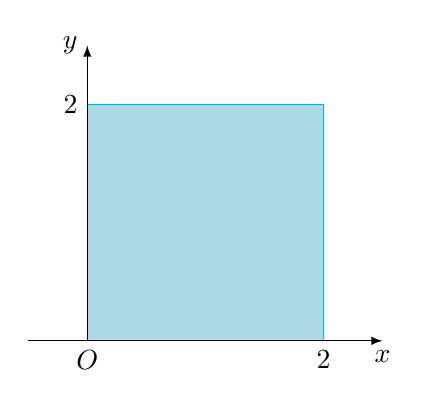
\begin{tikzpicture}[scale = 1.5]
                %画填充色快
                \filldraw[LightBlue] (0, 0) -- (2, 0) -- (2, 2) -- (0,2) -- cycle;
                \draw[cyan] (0, 0) -- (2, 0) -- (2, 2) -- (0,2) -- cycle;
                %画坐标系并标注
                \draw[-latex] (-0.5, 0) -- (2.5, 0) node[below] {$x$};
                \draw[-latex] (0, 0) -- (0, 2.5) node[left] {$y$};
                \node[below] at (0, 0) {$O$};
                %标注区域边界
                \node[below] at (2, 0) {$2$};
                \node[left] at (0, 2) {$2$};
            \end{tikzpicture}
        \end{center}
    \end{center}
    根据数学期望的定义,$X$ 的数学期望为
    $$
        \begin{aligned}
            E(X)
             & = \int_{-\infty}^{+\infty}\int_{-\infty}^{+\infty} xf(x,y) \,\mathrm{d}x\mathrm{d}y
            = \int_0^2 \mathrm{d}x\int_0^2\frac{x}{8}(x+y)\,\mathrm{d}y                                                 \\
             & = \int_0^2 \left.\left(\frac{x^2}{8}y + \frac{x}{8}\frac{y^2}{2}\right)\right|_{y=0}^{y=2} \,\mathrm{d}x
            = \int_0^2 \frac{x^2}{4} + \frac{x}{4} \,\mathrm{d}x                                                        \\
             & =\left.\left(\frac{x^3}{12} + \frac{x^2}{8}\right)\right|_{x=0}^{x=2}  = \frac{7}{6} .                   \\
        \end{aligned}
    $$
    $X^2$ 的数学期望为
    $$
        \begin{aligned}
            E(X^2)
             & = \int_{-\infty}^{+\infty}\int_{-\infty}^{+\infty} x^2f(x,y) \,\mathrm{d}x\mathrm{d}y
            = \int_0^2 \mathrm{d}x\int_0^2\frac{x^2}{8}(x+y)\,\mathrm{d}y                                                 \\
             & = \int_0^2 \left.\left(\frac{x^3}{8}y + \frac{x^2}{8}\frac{y^2}{2}\right)\right|_{y=0}^{y=2} \,\mathrm{d}x
            = \int_0^2 \frac{x^3}{4} + \frac{x^2}{4} \,\mathrm{d}x                                                        \\
             & = \left.\left(\frac{x^4}{16} + \frac{x^3}{12}\right)\right|_{x=0}^{x=2}  = \frac{5}{3}.                    \\
        \end{aligned}
    $$
    $XY$ 的数学期望为
    $$
        \begin{aligned}
            E(XY)
             & = \int_{-\infty}^{+\infty}\int_{-\infty}^{+\infty} xyf(x,y) \,\mathrm{d}x\mathrm{d}y = \int_0^2 \mathrm{d}x\int_0^2\frac{xy}{8}(x+y)\,\mathrm{d}y                      \\
             & = \int_0^2 \left.\left(\frac{x^2}{8}\frac{y^2}{2} + \frac{x}{8}\frac{y^3}{3}\right)\right|_{y=0}^{y=2}\mathrm{d}x = \int_0^2 \frac{x^2}{4} + \frac{x}{3} \,\mathrm{d}x \\
             & = \left.\left(\frac{x^3}{12} + \frac{x^2}{6}\right)\right|_{x=0}^{x=2}   = \frac{4}{3}.                                                                                \\
        \end{aligned}
    $$
    同理
    $$
        E(Y) = \frac{7}{6}, \quad E(Y^2) = \frac{5}{3}.
    $$
    根据数学期望的性质
    $$
        D(X)
        = E\left\{[X - E(X)]^2\right\}
        = E(X^2)-E^2(X)
        = \frac{5}{3}-\left(\frac{7}{6}\right)^2
        = \frac{11}{36}.
    $$
    $$
        D(Y)
        = E\left\{[Y - E(Y)]^2\right\}
        = E(Y^2)-E^2(Y)
        = \frac{5}{3}-\left(\frac{7}{6}\right)^2
        = \frac{11}{36}.
    $$
    根据协方差的定义
    $$
        \cov(X,Y)
        = E\{[X-E(X)][Y-E(Y)]\}
        = E(XY) - E(X)E(Y)
        = \frac{4}{3} - \frac{7}{6} \times \frac{7}{6}
        = -\frac{1}{36}.
    $$
    根据相关系数的定义和方差的性质
    $$
        \rho_{XY}
        = \frac{\cov(X,Y)}{\sqrt{D(X)}\sqrt{D(Y)}}
        = \frac{-\frac{1}{36}}{\sqrt{\frac{11}{36}}\sqrt{\frac{11}{36}}}
        = -\frac{1}{11}.
    $$
    根据方差的性质
    $$
        \begin{aligned}
            D(X+Y)
             & = E\left\{[(X+Y) - E(X+Y)]^2\right\}                                                          \\
             & = E\left\{[(X-E(X)) + (Y-E(Y))]^2\right\}                                                     \\
             & = E\left\{[X-E(X)]^2\right\} + E\left\{[Y-E(Y)]^2\right\} + 2E\left\{[X-E(X)][Y-E(Y)]\right\} \\
             & = D(X) + D(Y) + 2\cov(X,Y)                                                                    \\
             & = \frac{11}{36} + \frac{11}{36} + 2 \times \left(-\frac{1}{36}\right)                         \\
             & = \frac{5}{9}.
        \end{aligned}
    $$
\end{solution}



\begin{question}{题目33}
    设随机变量 $X \sim N(\mu, \sigma^2)$,$Y \sim N(\mu, \sigma^2)$,且设 $X,Y$ 相互独立,试求 $Z_1 = \alpha X + \beta Y$ 和 $Z_2 = \alpha X - \beta Y$ 的相关系数(其中 $\alpha, \beta$ 是不为零的常数).
\end{question}
\begin{solution}
    根据协方差的定义和数学期望的性质,结合 $X,Y$ 的独立性
    $$
        \begin{aligned}
            \cov(Z_1, Z_2)
            %& = E\left\{[Z_1-E(Z_1)][Z_2-E(Z_2)]\right\}                               \\
             & = E(Z_1Z_2) - E(Z_1)E(Z_2)                                                              \\
             & = E(\alpha^2X^2-\beta^2Y^2) - E(\alpha X + \beta Y)E(\alpha X - \beta Y)                \\
             & = \alpha^2E(X^2) - \beta^2E(Y^2) - [\alpha E(X) + \beta E(Y)][\alpha E(X) - \beta E(Y)] \\
             & = \alpha^2[E(X^2)-E^2(X)] - \beta^2 [E(Y^2)-E^2(Y)]                                     \\
             & = (\alpha^2 - \beta^2)\sigma^2.                                                         \\
        \end{aligned}
    $$
    根据方差的性质
    $$
        D(Z_1) = D(\alpha X + \beta Y)
        = \alpha^2D(X) + \beta^2D(Y)
        = (\alpha^2+\beta^2)\sigma^2.
    $$
    $$
        D(Z_2) = D(\alpha X - \beta Y)
        = \alpha^2D(X) + \beta^2D(Y)
        = (\alpha^2+\beta^2)\sigma^2.
    $$
    相关系数为
    $$
        \rho_{Z_1Z_2} = \frac{\cov(Z_1, Z_2)}{\sqrt{D(Z_1)}\sqrt{D(Z_2)}}
        = \frac{(\alpha^2 - \beta^2)\sigma^2}{\sqrt{(\alpha^2+\beta^2)\sigma^2}\sqrt{(\alpha^2+\beta^2)\sigma^2}}
        = \frac{\alpha^2-\beta^2}{\alpha^2+\beta^2}.
    $$
\end{solution}